\subsection{ImageNet}
\texttt{ImageNet}\autocite{imagenet_cvpr09} is an ongoing project, which aims to map images to features by means of crowd-sourcing the effort to label the dataset. 
The dataset consists of over 14M distinct images across 1000 main categories and additional subcategories/hierarchies. 
\begin{figure}[H]
    \centering
    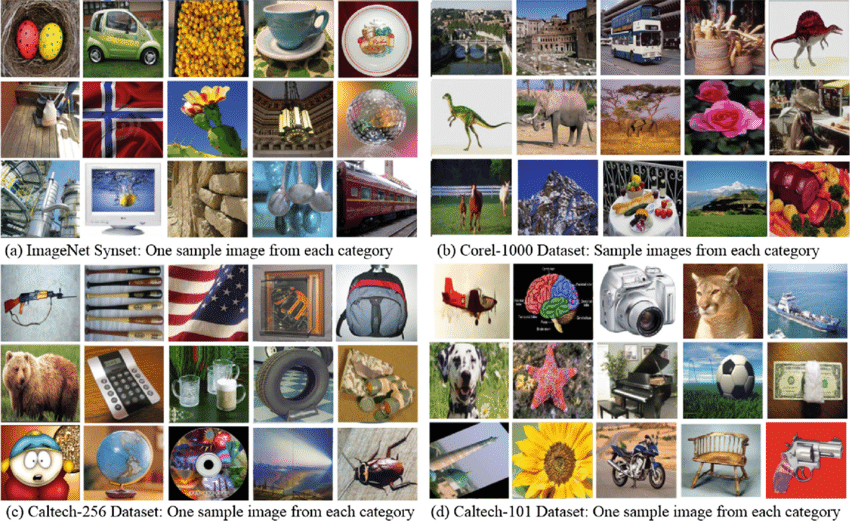
\includegraphics[scale=0.3]{pictures/random/imagenet}
    \caption{Example of ImageNet data. Image source: \autocite{imagenetex}}
    \label{fig:imagenetdata}
\end{figure}

\newline
ImageNet is a commonly used dataset for large-scale training of deep neural networks and serves as a benchmark in many computer vision publications.
Milestones in computer vision reached on the ImageNet Challenge(ILSVRC) involve work such as AlexNet in 2012, VGGNet\autocite{NIPS2012_4824} in 2014 and ResNet\autocite{ResNet2015} in 2015. 
\newline
Models trained on the ImageNet data may perform well in transfer learning tasks due to the large source domain, $\mathcal{D}_{S}$ - which should produce generalizable features. 
It may also be the case that such a model picks up on too general features and may not produce the features needed to distinguish more minute details in rooms such as door-frames or washing machines.
